 \documentclass[xcolor=table]{beamer}
\mode<presentation> {

% The Beamer class comes with a number of default slide themes
% which change the colors and layouts of slides. Below this is a list
% of all the themes, uncomment each in turn to see what they look like.

% \usetheme{default}
%\usetheme{AnnArbor}
%\usetheme{Antibes}
%\usetheme{Bergen}
%\usetheme{Berkeley}����JFIF����C
%\usetheme{Berlin}
%\usetheme{Boadilla}
%\usetheme{CambridgeUS}
%\usetheme{Copenhagen}
%\usetheme{Darmstadt}
%\usetheme{Dresden}
%\usetheme{Frankfurt}
%\usetheme{Goettingen}
%\usetheme{Hannover}
%\usetheme{Ilmenau}
% \usetheme{JuanLesPins}
% \usetheme{Luebeck}
% \usetheme{Madrid}
%\usetheme{Malmoe}
%\usetheme{Marburg}
%\usetheme{Montpellier}
\usetheme{PaloAlto}
%\usetheme{Pittsburgh}
%\usetheme{Rochester}
%\usetheme{Singapore}
%\usetheme{Szeged}
% \usetheme{Warsaw}

% As well as themes, the Beamer class has a number of color themes
% for any slide theme. Uncomment each of these in turn to see how it
% changes the colors of your current slide theme.

% \usecolortheme{albatross}
%\usecolortheme{beaver}
%\usecolortheme{beetle}
% \usecolortheme{crane}
%\usecolortheme{dolphin}
 \usecolortheme{dove}
% \usecolortheme{fly}
% \usecolortheme{lily}
% \usecolortheme{orchid}
% \usecolortheme{rose}
% \usecolortheme{seagull}
% \usecolortheme{seahorse}
% \usecolortheme{whale}
% \usecolortheme{wolverine}
% \usecolortheme{dracula}

%\setbeamertemplate{footline} % To remove the footer line in all slides uncomment this line
\setbeamertemplate{footline}[page number] % To replace the footer line in all slides with a simple slide count uncomment this line

%\setbeamertemplate{navigation symbols}{} % To remove the navigation symbols from the bottom of all slides uncomment this line
}

% \usepackage[demo]{graphicx}

\usepackage{polski}
\usepackage[utf8]{inputenc}
\usepackage{neuralnetwork}
\usepackage{adjustbox}

\usepackage[para,online,flushleft]{threeparttable}
\usepackage{enumitem}
\usepackage{pifont}
\usepackage[normalem]{ulem}
\usepackage{listings}
\usepackage{xcolor}
\usepackage{minted}

\setbeamertemplate{caption}[numbered]

\defbeamertemplate{description item}{align left}{\insertdescriptionitem\hfill}
\beamertemplatenavigationsymbolsempty
\setbeamertemplate{description item}[align left]

%----------------------------------------------------------------------------------------
%	TITLE PAGE
%----------------------------------------------------------------------------------------
\title[Cykl życia Obiektów]{Inicjalizacja i niszczenie obiektów w wybranym języku programowania.} % The short title appears at the bottom of every slide, the full title is only on the title page

\author{Patryk Lisik} % Your name
\institute[] % Your institution as it will appear on the bottom of every slide, may be shorthand to save space
{
  Uniwersytet Łódzki \\ % Your institution for the title page
}

\date{2023/24} % Date, can be changed to a custom date

\begin{document}

\begin{frame}
\titlepage
% Print the title page as the first slide
\end{frame}

\begin{frame}
    
\end{frame}

%----------------------------------------------------------------------------------
\section{Typ i obiekt}

\begin{frame}[containsverbatim]{Co to typ?}
    \begin{block}{Typ}
        Dane i zbiór operacji, które można na nich wykonać \cite{IBM-What-is-type}.
    \end{block}
    \begin{figure}
        \centering
    \begin{minted}{cpp}
    class LineFunction {
        double a, b; //dane

        // operajca
        double operator()(double x) const{ 
            return a * x + b;
        }
    };
    \end{minted}
    \caption{Przykład własnego typu w C++}
        \label{fig:cpp-operator-overload}
    \end{figure}

\end{frame}

\begin{frame}[containsverbatim]{Co to obiekt?}

    \begin{block}{Obiekt}
        Ukonkretnienie typu w postaci zaalokowanej pamięci. 
    \end{block}

    \begin{block}{Obiekt}
    \begin{figure}
        \centering
    \begin{minted}{cpp}
        LineFunction func{4.5, 2.1};
        double d = func(7.2);
    \end{minted}
    \end{figure}

    \end{block}
    
\end{frame}

\begin{frame}
    
\end{frame}

\section{Cykl życia obiektów w C++}




%----------------------------------------------------------------------------------------
%     class LineFucntion {
%         public:
%             double a, b; //dane

%         // operajca
%         double operator()(double x) const{ 
%             return a * x + b;
%         }
%     };


% int main(){
%     LineFucntion func{4.5, 2.1};
%     double d = func(7.2);
%     return 0;
% }

%----------------------------------------------------------------------------------------
\begin{frame}[containsverbatim]{Konstruktor}
    \begin{figure}
        \centering
        \tiny
    \begin{minted}{cpp}
    #include <cstdio>
    #include <algorithm>
    class LineFucntion {
        public:
            double a, b;
            //konstruktor
            LineFucntion(double a , double b){ 
                puts("Constructor");
                this->a=a;
                this->b=b;
            }

            // kontruktor kopiujący 
            LineFucntion(LineFucntion const & lf){
                 puts("Copy constuctor");
            }

            //destruktor
            ~LineFucntion(){
                puts("Destructor");
            }
        double operator()(double x) const{ return a * x + b;}
    };


    \end{minted}
        \label{fig:cpp-constructor}
        \caption{Jawnie zdefiniowany konstruktor w C++. Zgodnie z zasadą 0/3/5.}
    \end{figure}
    
\end{frame}

\begin{frame}[containsverbatim]{Type alokacji}
    \begin{figure}
        \centering
        \tiny
    \begin{minted}{cpp}
            int main(){
                LineFucntion func{4.5, 2.1};
                double d = func(7.2);
                puts("In between");
                return 0;
            }
    \end{minted}
        \label{fig:cpp-stack-allocation}
        \caption{Alokacja na stosie}
    \end{figure}
    
    \begin{figure}
        \centering
        \tiny
    \begin{minted}{cpp}
            int main(){
                LineFucntion* func = new LineFucntion(4.5, 2.1);
                double d = (*func)(7.2);
                puts("In between");
                delete func;
                return 0;
            }
    \end{minted}
        \label{fig:cpp-heap-allocation}
        \caption{Alokacja na stercie}
    \end{figure}
\end{frame}


\begin{frame}[containsverbatim]{ABI konstruktorów w C++ }

\begin{block}{Interfejs binarny aplikacji w c++}
    Kompilatory C++ są zgodne z Itanium C++ ABI \cite{itanium-abi}.
    Które definiuje następujące konstruktory i ich nazwy:

\begin{minted}{text}
<ctor-dtor-name>
::= C1# complete object constructor 
::= C2# base object constructor 
::= C3# complete object allocating constructor 
::= CI1 <base type>#complete inheriting constructor
::= CI2 <base type>#base inheriting constructor
::= D0# deleting destructor
::= D1# complete object destructor
::= D2# base object destructor
 \end{minted}
\end{block}
\end{frame}

\begin{frame}[containsverbatim]{Użycie konstruktorów z ABI}
    \begin{block}{}
     Konstruktor C1 jest używany gdy obiekt nie jest klasą pochodną \cite{IBM-Two-identical-constructor}.
     Konstruktor C2 jest używany gdy tworzony jest obiekt jest klasą pochodną. Kompilator zawsze emituje oba konstruktory. 
    \end{block}
    
    \begin{block}{}
     Konstruktor C3 nie jest nigdy generowany przez GCC \cite{gcc-constructor}.
    \end{block}

\begin{block}{}
    W C++ konstruktory domyślnie nie są dziedziczone.
    CI1 i CI2 są używane gdy w standardzie C++11 je dziedziczymy.
    \tiny
    \begin{minted}{cpp}
class A{
    public: 
        A(int x) {}
};

class B: public A{
     using A::A;
};
    \end{minted}
\end{block}

\end{frame}




\begin{frame}[containsverbatim]{Podwójne wywołanie destruktora?}
\tiny
\begin{block}{}
    ABI wymaga destruktora D1 i D2, które są tożsame w przypadku braku dziedziczenia.
\end{block}
    \begin{figure}
        \tiny
    \begin{minted}{cpp}
main:
//usunięta nieistotna czesc
        call    LineFucntion::LineFucntion(double, double) [complete object constructor]
        mov     rdx, QWORD PTR .LC4[rip]
        lea     rax, [rbp-48]
        movq    xmm0, rdx
        mov     rdi, rax
        call    LineFucntion::operator()(double) const
        movq    rax, xmm0
        mov     QWORD PTR [rbp-24], rax
        mov     edi, OFFSET FLAT:.LC5
        call    puts
        mov     ebx, 0
        lea     rax, [rbp-48]
        mov     rdi, rax
        call    LineFucntion::~LineFucntion() [complete object destructor]
        mov     eax, ebx
        jmp     .L9
        mov     rbx, rax
        lea     rax, [rbp-48]
        mov     rdi, rax
        call    LineFucntion::~LineFucntion() [complete object destructor]
//usunięta nieistotna czesc 
        \end{minted}
                \label{fig:cpp-constructor-asm}
                \caption{Wynik kompilacji kodu z rys. \ref{fig:cpp-stack-allocation} za pomocą GCC 13.3 z flagą -00}
        \end{figure}
\end{frame}


\begin{frame}[containsverbatim]{Alokacja i dealokacja na stercie}
    \begin{figure}
        \tiny
    \begin{minted}{cpp}
main:
//usunięta nieistotna czesc
        call    operator new(unsigned long)
        mov     rbx, rax
        mov     r13d, 1
        movsd   xmm0, QWORD PTR .LC2[rip]
        mov     rax, QWORD PTR .LC3[rip]
        movapd  xmm1, xmm0
        movq    xmm0, rax
        mov     rdi, rbx
        call    LineFucntion::LineFucntion(double, double) [complete object constructor]
        mov     QWORD PTR [rbp-40], rbx
        mov     rdx, QWORD PTR .LC4[rip]
        mov     rax, QWORD PTR [rbp-40]
        movq    xmm0, rdx
        mov     rdi, rax
        call    LineFucntion::operator()(double) const
        movq    rax, xmm0
        mov     QWORD PTR [rbp-48], rax
        mov     edi, OFFSET FLAT:.LC5
        call    puts
        mov     rbx, QWORD PTR [rbp-40]
        test    rbx, rbx
        je      .L6
        mov     rdi, rbx
        call    LineFucntion::~LineFucntion() [complete object destructor]
        mov     esi, 16
        mov     rdi, rbx
        call    operator delete(void*, unsigned long)
//usunięta nieistotna czesc 
        \end{minted}
                \label{fig:cpp-constructor-heap-asm}
                \caption{Wynik kompilacji kodu z rys. \ref{fig:cpp-stack-allocation} za pomocą GCC 13.3 z flagą -00}
        \end{figure}
\end{frame}

\begin{frame}{Alokacja pamięci}
    \begin{block}{Alokacja pamięci}
        Alokacja pamięci to rezerwacja przez system operacyjny pamięci dla procesu\cite{mmap-linux_man, virtual-alloc}.
        
        \textit{(Nie rozpatrujmy sytuacji gdy nie ma systemu operacyjnego)}
    \end{block}
    \begin{block}{POSIX}
        W systemach zgodnych z POSIX alokacja pamięci odbywa się poprzez  `mmap()` \cite{mmap-linux_man}.
    \end{block}

    \begin{block}{Windows}
        W systemach Windows alokacja pamięci odbywa się poprzez VirtualAlloc[memoryapi.h] \cite{virtual-alloc}.
    \end{block}
\end{frame}

\begin{frame}[containsverbatim]{Kolejność wywoływania konstruktorów}
\begin{minted}{cpp}
class ChildFucntion : public LineFucntion { 
    public:
ChildFucntion(double a, double b): LineFunction(a,b){
    puts("Child");}
    
ChildFucntion(ChildFucntion const & cf{
   puts("Child copy constuctor");
    }
~CholdFucntion(){puts("Child destructor");}
    }
\end{minted}
\begin{block}{}
    Najpierw wywoływany jest konstruktor rodzica.
\end{block}
\end{frame}
%----------------------------------------------------------------------------------------
\section{Automatyczne zarządzanie pamięcią w C++}

\begin{frame}{Unique\_ptr}
    \begin{block}{Własność w programowaniu}
        Własność określa kto jest odpowiedzialny za zwolnienie pamięci \cite{rust-ownership, cpp-unique-ptr}.
    \end{block}

    \begin{block}{}
        std::move informuje kompilator o możliwości przeniesienie zasobów już istniejącego obiektu.
    \end{block}
\end{frame}

%----------------------------------------------------------------------------------------
\begin{frame}{Shared\_ptr}
    \begin{block}{}
        std:shared\_ptr składa się z licznika referencji i właściwego wskaźnika. 
        Podczas kopi licznik referencji jest zwiększany, a podczas wywołania destruktora zmniejszany. 
        Przy wywołaniu ostatniego destruktora pamięć jest zwalniana \cite{cpp-shared-ptr}. 
    \end{block}
\end{frame}

%----------------------------------------------------------------------------------------
\begin{frame}{Problem cyklicznych referencji}
    \begin{figure}
        \centering
        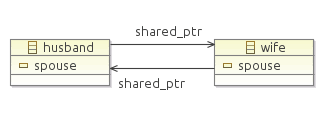
\includegraphics[width=7cm]{cyclic_ref.png}
        \caption{Problem cyklicznych referencji gdzie pamięć nigdy nie jest zwalniana. Źródło: \cite{weak-ptr-vs-magazine}}
        \label{fig:enter-label}
    \end{figure} 

\begin{block}{std::weak\_ptr}
    Rozwiązaniem problemu cyklicznych referencji jest referencja słaba(std::weak\_ptr) która nie powoduje inkrementacji licznika referencji. Nie gwarantuje one że obiekt nie został już usunięty \cite{weak-ptr-vs-magazine, cpp-weak-ptr}. 
\end{block}
\end{frame}



\section{Odśmiecanie Garbage Collector}

\begin{frame}{Oznacz i zmieć (ang. \textit{mark and sweep})}
    \begin{block}{Faza mark}
        Przeszukujemy "w głąb" graf obiektów i oznaczamy każdy obiekt do którego dotarliśmy \cite{mark-and-sweep}. 
    \end{block}
    \begin{block}{Faza sweep}
        Usuwamy obiekty nieoznaczone.
    \end{block}
        \begin{block}{Faza compact(Opcjonalna)}
        Obiekty przesuwane są blisko siebie w pamięci.
    \end{block}

    \begin{block}{Krytyka}
    \begin{itemize}
        \item Jest to bardzo wolny algorytm, który wymaga zatrzymania przetwarzania do działania (ang. \textit{stop the world GC}).
        \item  Bez fazy compact powoduje dużą fragmentację pamięci. 
    \end{itemize}
    \end{block}
\end{frame}


\begin{frame}{Inne rodzaje odśmiecaczy/garbage collectorów}
\begin{block}{}
Generacyjny \\
Trzy kolorowy  \\
Arenowy
\end{block}


\end{frame}

\begin{frame}[allowframebreaks]{Literatura}

\begin{thebibliography}{99}
\bibliographystyle{ieeetr}
\bibliography{refs} 
\end{thebibliography}

\end{frame}
\end{document}
